%% LyX 2.0.0 created this file.  For more info, see http://www.lyx.org/.
%% Do not edit unless you really know what you are doing.
\documentclass[12pt,a4paper]{article}
\usepackage{amsmath}
\usepackage{amssymb}
\usepackage{fontspec}
\setmainfont[Mapping=tex-text]{Times New Roman}
\usepackage{listings}
\usepackage{array}
\usepackage{float}
\usepackage{units}
\usepackage{multirow}
\usepackage{graphicx}
\usepackage{setspace}
\usepackage{esint}
\onehalfspacing

\makeatletter

%%%%%%%%%%%%%%%%%%%%%%%%%%%%%% LyX specific LaTeX commands.
\pdfpageheight\paperheight
\pdfpagewidth\paperwidth

%% Because html converters don't know tabularnewline
\providecommand{\tabularnewline}{\\}

%%%%%%%%%%%%%%%%%%%%%%%%%%%%%% User specified LaTeX commands.
\usepackage[left=25mm,right=25mm,top=28mm,bottom=20mm,headsep=4mm,footskip=8mm,voffset=-4mm]{geometry}
\usepackage{fancyhdr} %页眉页脚
\usepackage[square,super,comma,sort,compress]{natbib} %文献格式
\usepackage{titletoc}
\usepackage{titlesec}
\usepackage[dvipsnames,svgnames,x11names]{xcolor} %彩色工具
\usepackage[CJKbookmarks=true]{hyperref}
%首行缩进
\parindent=2em
%% 定义正文字体
\usepackage{fontspec}
%\usepackage[slantfont,boldfont]{xeCJK}
\usepackage[BoldFont,CJKnumber]{xeCJK}
\setmainfont{Times New Roman}
\setmonofont{Consolas}
%\setmonofont{Courier New}
\setCJKmainfont{SimSun}
\setCJKfamilyfont{song}{SimSun}
\setCJKfamilyfont{hei}{SimHei}
\newcommand\song{\CJKfamily{song}}
\newcommand\hei{\CJKfamily{hei}}

\renewcommand{\baselinestretch}{1.25}
\usepackage{xunicode}% provides unicode character macros
\usepackage{xltxtra} % provides some fixes/extras


% 重定义字号命令
\newcommand{\xiaochu}{\fontsize{30pt}{40pt}\selectfont}    % 小初, 1.5倍行距
\newcommand{\yihao}{\fontsize{26pt}{36pt}\selectfont}    % 一号, 1.4倍行距
\newcommand{\erhao}{\fontsize{22pt}{28pt}\selectfont}    % 二号, 1.25倍行距
\newcommand{\xiaoer}{\fontsize{18pt}{18pt}\selectfont}    % 小二, 单倍行距
\newcommand{\sanhao}{\fontsize{16pt}{24pt}\selectfont}    % 三号, 1.5倍行距
\newcommand{\xiaosan}{\fontsize{15pt}{22pt}\selectfont}    % 小三, 1.5倍行距
\newcommand{\sihao}{\fontsize{14pt}{21pt}\selectfont}    % 四号, 1.5倍行距
\newcommand{\banxiaosi}{\fontsize{13pt}{19.5pt}\selectfont}    % 半小四, 1.5倍行距
\newcommand{\xiaosi}{\fontsize{12pt}{15pt}\selectfont}    % 小四, 1.25倍行距
\newcommand{\dawuhao}{\fontsize{11pt}{11pt}\selectfont}    % 大五号, 单倍行距
\newcommand{\wuhao}{\fontsize{10.5pt}{10.5pt}\selectfont}    % 五号, 单倍行距
\newcommand{\xiaowu}{\fontsize{9pt}{9pt}\selectfont}    % 小五号, 单倍行距


\renewcommand{\title}[1]{\def\ECUST@title{#1}}
\def\ECUST@title{}
\def\mainmatter{\fancypagestyle{plain}{}
    \pagestyle{fancy}
    \fancyhead[LO,RE]{\xiaowu{\ECUST@title}}%
    \fancyhead[RO,LE]{\wuhao{\thepage}}%
    \fancyfoot{}%

}
\renewcommand{\contentsname}{\hei\xiaoer 目~录}
\setcounter{tocdepth}{2}\setcounter{secnumdepth}{4}
\titlecontents{section}[12bp]{\vspace{0pt}}
    {\hei\sihao\thecontentslabel\quad}{}
    {\hspace{.5em}\titlerule*[10pt]{$\cdot$}\contentspage}
\titlecontents{subsection}[12bp]{\vspace{0pt}}
    {\hei\xiaosi\thecontentslabel\quad}{}
    {\hspace{.5em}\titlerule*[10pt]{$\cdot$}\contentspage}

%% 正文标题格式
\titleformat{\section}[hang]{\centering\hei\xiaoer}{\thesection{}}{1em}{}
\titleformat{\subsection}[hang]{\song\sihao}{\thesubsection}{0.5em}{}
\titleformat{\subsubsection}[hang]{\hei\xiaosi}{\thesubsubsection}{0.5em}{}
\titlespacing{\section}{0bp}{0bp}{12bp}
\titlespacing{\subsection}{0bp}{12bp}{0bp}
\titlespacing{\subsubsection}{0bp}{12bp}{0bp}
   
% 图表定义
\renewcommand{\figurename}{\bfseries \song \xiaowu 图}
\numberwithin{figure}{section}
\renewcommand{\tablename}{\bfseries \song \xiaowu  表}
\numberwithin{table}{section}
\renewcommand{\thefigure}{\thesection-\arabic{figure}}
\renewcommand{\thetable}{\thesection.\arabic{table}}
\renewcommand{\lstlistingname}{\bfseries \song \xiaowu 算法}
\def\thelstlisting{\thesection.\arabic{lstlisting}}

%\makeatletter
%\@addtoreset{figure}{section}
%\makeatother


%公式按章编号

\numberwithin{equation}{section}
\renewcommand{\theequation}{\thesection-\arabic{equation}} 


%% 引用文献格式
%\let\textcite=\cite
%\renewcommand{\cite}[1]{\textsuperscript{\xiaosihao\textcite{#1}}}
\renewcommand\refname{\vspace{0pt}参考文献\vspace{12pt}}

%% 中文摘要和关键词
\newenvironment{cnabstract}[1][]{%
        \thispagestyle{plain}%
    \fancyfoot{}%
    \def\ECUST@keywords{#1}%
        \vspace*{102bp}%
        \begin{center}%
        {\hei\xiaoer 摘要}%
        \end{center}
        \vspace{12bp}%
    \par%
}{%
    \par%
    \vspace{12bp}%
    \noindent%
    {\quad\quad\hei\xiaosi 关键词:}\quad{\ECUST@keywords}%
    %\let\ECUST@keywords=\relax%
    \clearpage%
    %\setcounter{page}{0}%
}


%% 英文摘要和关键词
\newenvironment{enabstract}[1]{%
        \thispagestyle{plain}%
    \fancyfoot{}%
    \def\ECUST@keywords{#1}%
        \vspace*{102bp}%
        \begin{center}%
        {\bfseries\xiaoer Abstract}%
        \end{center}
        \vspace{12bp}%
    \par%
}{%
    \par%
    \vspace{12bp}%
    \noindent%
    { \quad \quad \bfseries\xiaosi Keywords:}\quad{\ECUST@keywords}%
    %\let\ECUST@keywords=\relax%
    \clearpage%
    %\setcounter{page}{0}%
}



%一些行距
\makeatletter
\def\enumerate{%
 \ifnum \@enumdepth >\thr@@\@toodeep\else
   \advance\@enumdepth\@ne
   \edef\@enumctr{enum\romannumeral\the\@enumdepth}%
     \expandafter
     \list
       \csname label\@enumctr\endcsname
       {\usecounter\@enumctr\def\makelabel##1{\hss\llap{##1}}%
         \addtolength{\parsep}{0.25ex}
         \addtolength{\itemsep}{-8pt} %%%%
         \addtolength{\topsep}{-8pt}
         }
 \fi}
\makeatother

\makeatletter
\def\itemize{%
 \ifnum \@itemdepth >\thr@@\@toodeep\else
   \advance\@itemdepth\@ne
   \edef\@itemitem{labelitem\romannumeral\the\@itemdepth}%
   \expandafter
   \list
     \csname\@itemitem\endcsname
     {\def\makelabel##1{\hss\llap{##1}}%
         \addtolength{\parsep}{0.25ex}
         \addtolength{\itemsep}{-8pt} %%%%
         \addtolength{\topsep}{-8pt}
         } %%%%
 \fi}
\makeatother


%代码列表样式
\usepackage{color}
\lstset{
         frame=leftline,
         extendedchars=true,
         breaklines=true,
         keywordstyle=\color{blue},
         stringstyle=\color{red},
         showspaces=false,
         showtabs=false,
         backgroundcolor=\color{lightgray},
         showstringspaces=false
}

\hypersetup{pdftitle={面板数据的非参数回归估计及其R语言实现和应用},
 pdfauthor={姜叶飞},
 pdfkeywords={面板数据 , 非参数计量经济学 , R语言 , 弹性影响}}

\makeatother

\usepackage{xunicode}
\usepackage{polyglossia}
\setdefaultlanguage{}
\begin{document}
\title{面板数据的非参数回归估计及其R语言实现和应用}
\pagenumbering{Roman}
\begin{cnabstract}[\xiaosi{面板数据 , 非参数计量经济学 , R语言 , 弹性影响}] 
\xiaosi{本文基于面板数据的非参数回归估计进行了实例研究以及R语言算法的实现}
\end{cnabstract} 
\begin{enabstract}{\xiaosi{Panel Data , Nonparametric Econometrics , R-Language , Elasticity Effect}}     
\xiaosi{This paper's analysis is based on the Nonparametric Regression Estimate theory of Panel Data, and also includes a Example and a achievement of R-Language algorithm. } 
\end{enabstract} 

\tableofcontents{}

\pagebreak{}

\pagenumbering{arabic} 
\setcounter{page}{1} 
\mainmatter


\section{引言}


\subsection{研究背景}


\subsubsection{非参数计量经济学}

计量经济学(Econometrics)作为经济学科的一个分支学科,在$20$世纪$20$年代末由R.Frish创立,经过$40$多年的发展,其经典理论方法已经成熟。自$20$世纪$70$年代以来,随着经济活动的复杂性增强和计量经济学应用领域的扩展,计量经济学理论方法得到了很大的发展。除了$2000$年诺贝尔经济学奖获得者J.J.Heckman对选择性样本模型理论的发展和D.L.Mcfadden对离散选择模型理论的发展,以及以此开创的微观计量经济学之外,宏观领域中动态计量经济学模型理论方法的发展是这个阶段最重要的部分,该方法以非参数模型理论方法为基础,并形成了较为完整的内容体系,构成了现代计量经济学的主要部分\cite{yaz2003}。然而到目前为止,它们仍旧处于新的领域,尚在研究和发展之中。因此,本文希望在前人研究的基础上,试图对它们的发展做出一点贡献。

\subsubsection{面板数据的非参数模型}

在一般模型中,时间序列数据或截面数据都是一维数据。时间序列数据是变量按时间得到的数据;截面数据是变量在固定时间点的一组数据。面板数据则是同时在时间和截面上取得的二维数据。所以,面板数据(Panel
Data)也称作时间序列与截面混合数据(Pooled Time Series and Cross Section Data)。也就是说,面板数据是截面上个体在不同时间点上重复观测的数据。其中,对一部分家庭或个体进行跟踪调查来获得的个体调查数据通常称为微观面板,所收集的数据特点是个体数$N$较大(通常是几百或几千个),而时期数$T$较短(最少是两年,最长不超过$10$年或$20$年)。而宏观面板通常涉及一段时期内不同国家的数据,这类数据一般具有适度规模的个体$N$(从$7$到$200$不等),时期数$T$一般在$20\thicksim60$年之间。因此,微观和宏观的面板要求使用不同的计量方法,例如,微观面板必须研究$T$固定而$N$较大时的渐进特性,而宏观面板的渐进特性则是指$T$和$N$都较大时的情况。还有,对于宏观面板,当时间序列较长时需要考虑数据的非平稳问题,如单位根、结构突变以及协整等;而微观面板不需要处理非平稳问题,特别是每个家庭或个体时期数$T$较短时。另外,在处理宏观面板时必须考虑国家之间的相关性,而在微观面板中,如果个体是随机抽样产生,则个体之间不大可能存在相关性,因此不需要考虑相关性问题。

在Hsiao(2003)\cite{hsiao2003analysis}的文章中给出了使用面板数据的一些优点:


\begin{itemize}
\item 可以控制个体异质性。面板数据表明个体、企业、州或国家之间都存在异质性。时间序列和横截面分析没有控制这种异质性,因此其结果很可能是有偏的。
\item 面板数据具有更多的信息,更大的变异,变量之间更弱的共线性,更大的自由度以及更高的效率。
\item 面板数据更适合于研究动态调整的过程。因为表面上相对稳定的横截面分布事实上隐藏了许多变化,失业的交替、工作的轮换、居住地的迁移和收入的波动等更适合于用面板数据研究。而且如果这种面板数据的时期数足够长,它们还能清楚地表明对经济政策变化的调整速度。
\item 面板数据还可以识别、测量单纯使用横截面或时间序列数据无法估计的影响。
\item 与纯横截面数据或时间序列数据相比,面板数据模型允许我们构建并检验更复杂的行为模型。
\item 基于个体、企业或家庭所收集的微观面板数据与在宏观层次上所收集的类似变量相比更加准确,而且还可能消除企业或个体数据加总所导致的偏倚。
\item 一般宏观面板数据中时间序列的时期数较长,而且与时间序列分析中进行单位根检验遇到的非标准分布问题不同,面板单位根检验通常具有标准的渐进分布。
\end{itemize}


但是,Baltagi(1995)\cite{baltagi1995econometric}也提到面板数据同样也存在这一些局限性:


\begin{itemize}
\item 调查设计和数据收集问题。这些问题包括:覆盖面问题(样本没有覆盖研究总体)、不响应问题(由于回答者的不合作或提问者的失误)、回忆问题(回答者的记忆不准确)、采访的频率问题、采访的时间间隔问题、询问的时间问题、界限使用问题和样本期内的偏倚问题。
\item 测量误差的扭曲。横截面数据的使用者没有别的选择,只能相信得到的结果,而面板数据使用者就可以通过对比间隔时间的调查来检查是否存在不一致性。这就能提醒面板数据的使用者注意测量误差的问题。
\item 选择问题。自选择、未回答和样本流失都对面板数据的使用有一定的限制。
\item 时间维度短。因为微观面板通常使用的是年度数据,每个个体的时期数较短,也就意味着渐进分析主要依赖个体数趋于无穷。但如果增加面板的时期数不仅增加成本,而且还会增加样本流失的可能性以及计算难度。
\item 截面相关性。国家或地区的宏观面板数据,如果时间序列较长而且没有考虑到国家之间的相关性就对导致错误的推断结论。因此,一般还需对截面数据的相关性进行单位根检验。
\end{itemize}


面板数据计量经济模型和其他截面或时间序列模型之间的一个重要差别是它允许截面或时间非均匀分布的存在。在此框架下大多评估两种模型,一种是固定效应模型,另一种是随机效应模型,也就是把原来(固定)的回归系数看作是随机变量,一般都是假设是来自正态分布来进行估计。这两种模型都可以控制分布的不均匀性。至于哪种应该在论文应用暂时还没有一个统一的规定,Maddala(1987)\cite{maddala1987recent}的文章中就固定和随机效应模型的评估给出了一个很好系数集。此外,计量经济学中的固定效应模型的工作最初由Mundlak(1961)\cite{mundlak1961empirical}和Hoch(1962)\cite{hoch1962estimation}发起,然而随机效应模型的研究由Balestra和Nerlove(1966)\cite{balestra1966pooling}提出并在Wallace与Hussain(1969)\cite{wallace1969use}、Maddala(1971)\cite{maddala1971use}、Nerlove(1971)\cite{nerlove1971note}以及Fuller与Battese(1973)\cite{fuller1973transformations}的研究中得到了进一步发展。并且从那时开始,大量的相关面板数据计量经济学论文开始发表出来,比如说由Heckman与Singer(2008)\cite{heckman2008longitudinal}、Hsiao(1985)\cite{hsiao1985benefits}和Baltagi(1995)\cite{baltagi1995econometric}等的相关著作;以及由Maddala(1987)\cite{maddala1987recent}和Baltagi(1996)\cite{baltagi1996nonparametric}做的相关方面的调查报告;在Matyas与Sevestre(1996)\cite{matyas1996econometrics}也出版了一本将近$900$页的手册以及Pesaran与Smith(1995)\cite{pesaran1995estimating}和Harris与Matyas(1996)\cite{harris1996comparative}的文章,这些文章都对动态面板数据模型理论的发展做了重要的贡献。以上述文件为背景,本文采用非参数模型来研究面板数据,该模型是基于Ullah和Roy(1998)《应用计量经济学手册》\cite{ullah1998handbook}中的相关模型来进行设定、推导和实现。


\subsection{R语言概述}

R语言是主要用于统计分析、绘图的语言和操作环境。R本来是由来自新西兰奥克兰大学的Ross Ihaka和Robert Gentleman开发。现在由“R开发核心团队”负责开发。R是基于S语言的一个GNU项目,所以也可以当作S语言的一种实现,通常用S语言编写的代码都可以不作修改的在R环境下运行。R的语法也同样是来自于Scheme\cite{rwiki}。

R语言给我们提供了一套完整的数据处理、计算和制图软件系统。其功能包括:


\begin{itemize}
\item 有效的数据存储和处理功能
\item 数组运算工具(其向量、矩阵运算方面功能尤其强大)
\item 拥有完整体系的数据分析工具
\item 为数据分析和显示提供的强大图形功能
\item 一套(源自S语言)完善、简单、有效的编程语言(包括条件、循环、自 定义函数、输入输出功能)。
\end{itemize}


R的定位是一个完善、统一的系统,而非其他数据分析软件那样作为一个专门、不灵活的附属工具。R很适合被用于发展中的新方法所进行的交互式数据分析。由于R是一个动态的环境,所以新发布的版本并不总是与之前发布的版本完全兼容。某些用户欢迎这些变化因为新技术和新方法的所带来的好处;有些则会担心旧的代码不
再可用。简而言之,R是GUI加上全球各地各种职业的个人和团体编写的包(Packages)组成的一个环境,使用者可以随时添加、删除以及更新这些包。从而在应用中,R并不仅仅是局限于普通的统计软件。因此选用R作为本次模型的实现环境会有较好的通用性和自由性。

\newpage{}


\section{参数模型与非参数模型的比较分析}


\subsection{计量经济参数模型简析}

在日常生活以及经济活动中,我们常常需要研究生产投入与产出之间的关系。例如,在宏观方面,以$Y=A(t)L^{\alpha}K^{\beta}\mu$为基本形式的Cobb-Douglas生产函数通过分析两者的关系,分析并预测了各个国家、地区的工业系统或大企业的产出水平;在微观方面,商品消费支出和收入之间关系(或恩格尔曲线)的研究也对两者之间的关系进行分析和预测以商品消费支出和收入之间关系为例,Working(1943)\cite{working1943statistical}、Leser(1963)\cite{leser1963forms}的实证研究表明,消费支出份额关于总支出的线性参数恩格尔曲线模型(Workling-Leser模型)可以较好地拟合其实际样本数据,模型形式如下:

\begin{equation}
w_{k}=\xi_{k}+\beta_{k}\log M
\end{equation}


其中,$w_{k}$是商品类$k$的消费支出$m_{k}$占总消费支出$M$的比例,$\xi_{k}$是与价格有关的常数,$\log$指以$e$为底的对数(下同)。这样表示的恩格尔曲线不但可以很好地拟合实际数据,而且还有一定的微观基础:它是几乎理想需求系统(AIDS)在价格给定的情况下的一个特例(详见Deaton与Muellbauer(1980)\cite{deaton1980almost}的结论)。参照周先波与田凤平(2008、2009)\cite{zxb2009,zxb20081}的研究结果可知,Working-Leser参数模型设定的总消费支出的对数和各类商品消费份额之间的关系是线性的。较强线性约束使其不一定能很好地描绘所有的数据。与传统非参数核估计进行比较,使用非参数估计方法拟合的图形比参数估计拟合的图形更好地反映了两变量之间的变化趋势及特征。在下面的章节中我们将通过一组数据比较参数估计和非参数估计的拟合效果。


\subsection{截面数据非参数Nadaraya-Watson核估计概述}

假设$Y$为被解释变量,$\boldsymbol{X}=\left(X_{1},\cdots,X_{q}\right)$为解释变量向量,是影响$Y$的$q$个重要因素。给定样本观测值$(Y_{1},\boldsymbol{X_{1}})$,$(Y_{2},\boldsymbol{X_{2}})$,$\cdots$,$(Y_{n},\boldsymbol{X_{n}})$,假定$(Y_{i},\boldsymbol{X_{i}})$独立同分布(下面简称i.i.d),建立非参数回归模型:

\begin{equation}
Y_{i}=m(\boldsymbol{X_{i}})+u_{i}
\end{equation}


其中,$m(\cdot)$是未知的函数,$m(\boldsymbol{X_{i}})=E(Y_{i}\mid\boldsymbol{X_{i}})$,$\varepsilon_{i}$是均值为零、方差为$1$且与$\boldsymbol{X_{i}}$独立的序列,随机误差项$u_{i}=\sigma(\boldsymbol{X_{i}})\varepsilon_{i}$,且$E(u_{i})=0$,$E(Y_{i})=m(\boldsymbol{X_{i}})$。则此时回归函数$m(x)$的核估计$\hat{m}_{n}(x)$为最小化:

\begin{equation}
\sum_{i=1}^{n}\left(Y_{i}-m(x)\right)^{2}K\left(\frac{\boldsymbol{X_{i}}-x}{h_{n}}\right)\label{eq:1}
\end{equation}


其中,$h_{n}$为窗宽,$K\left(\cdot\right)$为满足$K\left(u\right)\geq0$,$\int K\left(u\right)du=1$,$\int K\left(u\right)udu=0$的核函数。于是,我们可以得到公式(\ref{eq:1})的核估计的表达式为:

\begin{equation}
\hat{m}_{n}\left(x\right)=\frac{\sum_{i=1}^{n}K\left(\frac{\boldsymbol{X_{i}}-x}{h_{n}}\right)Y_{i}}{\sum_{i=1}^{n}K\left(\frac{\boldsymbol{X_{i}}-x}{h_{n}}\right)}\label{eq:2}
\end{equation}



\subsection{对比分析}

从公式(\ref{eq:2})中可以看出,核估计相当于作局部加权的最小二乘估计。那么,经典参数最小二乘估计与Nadaraya-Watson核估计在拟合效果上到底有多大差别呢?下面我们将通过使用一组数据来对其进行比较。

在R里面的MASS包中,我们可以找到一组名为mcycle的用来测试在事故发生时的摩托车加速度和时间的数据\cite{mcycle}。其中横轴为时间$X_{i}/ms$,纵轴为加速度$Y_{i}$。通过下列算法进行拟合。其中,线性回归选择使用stats包中的lm()函数,非参数回归选择使用KernSmooth包中的dpill函数确定窗宽,核函数选择Gauss核的locpoly函数进行拟合,具体算法见算法\ref{lis:mcycle}。

\begin{lstlisting}[caption={mcycle数据拟合},label={lis:mcycle},basicstyle={\tiny\ttfamily},breaklines=true,frame=leftline,language=R,numbers=left]
require(KernSmooth) 
require(MASS) 
data(mcycle) 
attach(mcycle) 
x <- times 
y <- accel
#线性 
plot(x,y) 
fit <- lm(y~x) 
abline(fit, lty=1, col='red', lwd=2) 
#非参 
plot(x,y) 
h=dpill(x,y) 
fit <- locpoly(x,y,kernel="normal",bandwidth=h,)
lines(fit,col='red')
\end{lstlisting}


\begin{figure}[H]
\begin{centering}
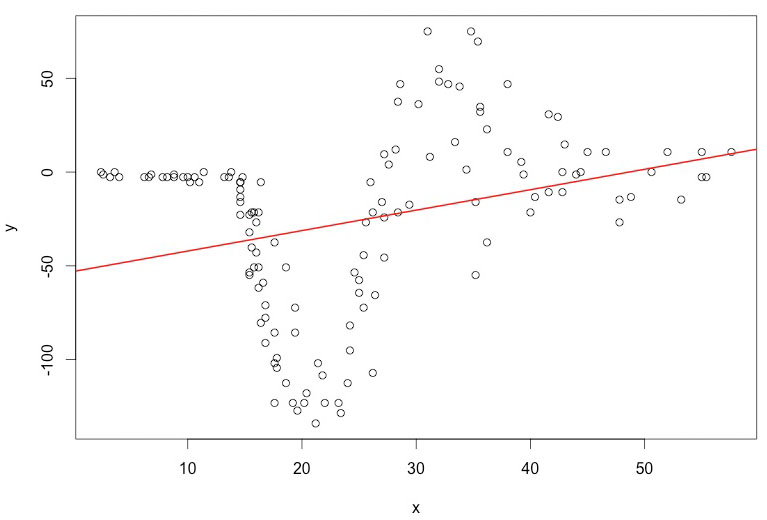
\includegraphics[width=14cm]{figure/mcyclelm}
\par\end{centering}

\caption{摩托车数据及其线性拟合图\label{fig:=006469=006258=008F66=006570=00636E=0053CA=005176=007EBF=006027=0062DF=005408=0056FE}}
\end{figure}


\begin{figure}[H]
\begin{centering}
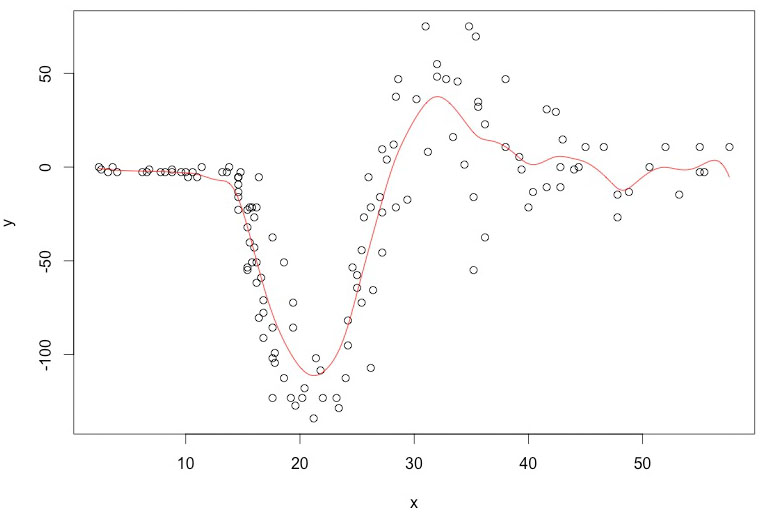
\includegraphics[width=14cm]{figure/mcycleloc}
\par\end{centering}

\caption{摩托车数据的非参数回归拟合图\label{fig:=006469=006258=008F66=006570=00636E=007684=00975E=0053C2=006570=0056DE=005F52=0062DF=005408=0056FE}}
\end{figure}


计算得到线性回归的拟合结果见图\ref{fig:=006469=006258=008F66=006570=00636E=0053CA=005176=007EBF=006027=0062DF=005408=0056FE},非参数回归见图\ref{fig:=006469=006258=008F66=006570=00636E=007684=00975E=0053C2=006570=0056DE=005F52=0062DF=005408=0056FE}。从这些图中我们可以清楚地看到,$Y_{i}$与$X_{i}$的关系是非线性关系,$ $给定已知的线性函数,拟合效果很差;即使使用其他已知的非线性函数,$Y_{i}$与$X_{i}$的拟合效果也显然不能令人满意。而在图\ref{fig:=006469=006258=008F66=006570=00636E=007684=00975E=0053C2=006570=0056DE=005F52=0062DF=005408=0056FE}中的非参数拟合图中我们可以看到非参数回归有很好的拟合效果,可以真实反映$Y_{i}$与$X_{i}$的实际关系(在不同的核函数和窗宽的选择下,拟合效果也有一定的差异)。$ $

\newpage{}


\setlength{\bibsep}{0.25ex}  %参考文献行距 

\phantomsection\addcontentsline{toc}{section}{\vspace{6pt}\sihao\hei 参考文献}

\bibliographystyle{ECUST}
\bibliography{Reference}


\newpage{}

\phantomsection\addcontentsline{toc}{section}{\sihao\hei 致谢}


\section*{致谢}

四年的大学生活在论文结束的这一刻也走到了尽头,我即将离开我的母校,开始新的人生和新的生活。


\end{document}
